The \textit{navigation} module is responsible for navigation the user from their current location to their desired location.  \\
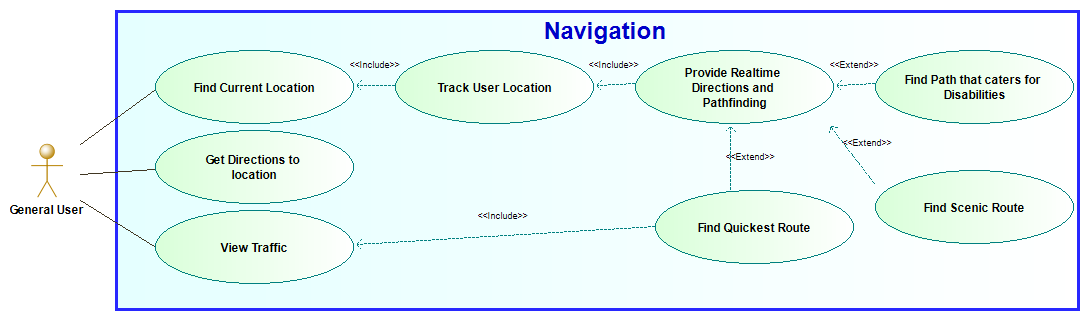
\includegraphics[width=\textwidth]{images/Navigation_Use_Case_Diagram.png}

\begin{center}
	Figure 7: Navigation Module Use Case
\end{center}

{The navigation system will use Wi-Fi to locate the general user's current location, this functionality will be extended in the use case where the system must track the user through their traversal on campus. The navigation subsystem will then also allow the general user to directed along a route or path to locations that they search for. There will be special use case instances where the routes plotted by the navigation system will be altered based on criteria set by the user, such as catering for disabilities. The navigation system will also allow general users to search view heat maps of campus and use this information in the routes that the system plots for them.}
